  \documentclass[a4j,twocolumn]{jsarticle}
  \usepackage[dvipdfmx]{graphicx}
  \usepackage{url}

  \setlength{\textheight}{275mm}
  \headheight 5mm
  \topmargin -30mm
  \textwidth 185mm
  \oddsidemargin -15mm
  \evensidemargin -15mm
  \pagestyle{empty}


  \begin{document}

  \title{旅行計画アプリの開発}
  \author{情報科学科 \hspace{5mm} 37022463 \hspace{5mm} 西谷研究室 山本果音}
  \date{}

  \maketitle


\section{序論}
\label{sec:org1c60c1a}
修学旅行などにおいて,参加者に対して事前に配布されるしおりは,旅程の把握や所持品の確認,集合時間の共有などを目的とした重要な情報媒体である.
近年では,紙媒体に代わりスマートフォンなどを用いて旅行情報を閲覧・共有するニーズが高まっており,これに応える形で旅しお[1]などのWebサービスが登場している.
しかし,旅行のプランニング用途で使用する場合,以下のような課題が存在する.
\begin{enumerate}
\item 図1のとおり,履歴には作成日・更新日が表示される一方で,旅行日程が時系列で整理されておらず,旅行の実施状況が視覚的に困難である.
\item 作成した地図をタイトルから直接検索する機能がなく,過去の旅行記録を振り替える際にスクロールをして探す不便が生じる.
\item 地図が表示されないため,目的地が視覚的に理解しにくい.
\end{enumerate}
結果として,利用者は外部ツールや手作業によって不足機能を補う必要があり,利便性や効率性に課題が残る.
そこで本研究では,時系列での視覚的把握を可能にするとともに,旅行記録に対してキーワードによる検索・絞り込みが可能な履歴管理機能を統合した旅行プランニングアプリの開発を目指す.


\begin{figure}[htbp]
\centering
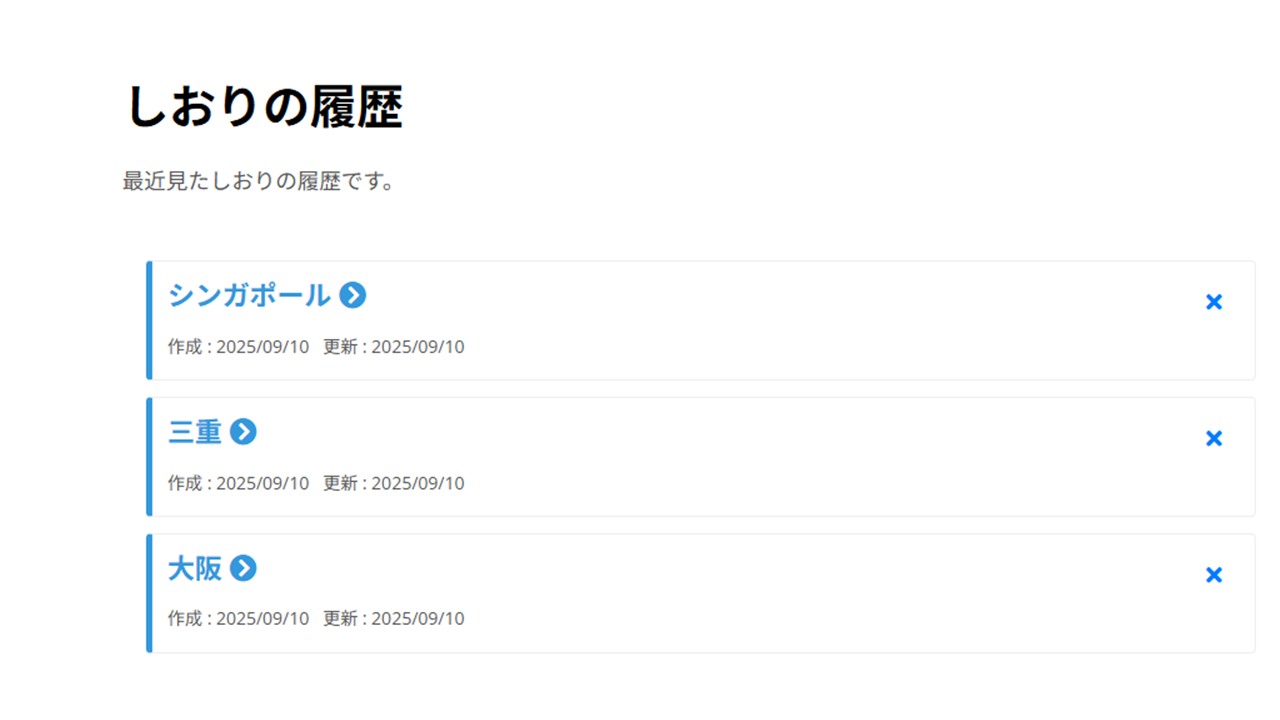
\includegraphics[width=7cm]{./figs/rireki1.png}
\caption{\label{fig:orgf0549a5}旅しおで作成したしおりの履歴表示画面.}
\end{figure}


\section{開発手法}
\label{sec:org604f3b5}
開発環境としてDjango[2]を選定した.
Djangoの利点は以下の2つである[3].
\begin{enumerate}
\item 迅速な開発が可能.
\item フォーム作成が容易にできる.
\end{enumerate}
また開発はPython, HTML, JavaScript, CSSを使用し、UIライブラリとしてはBootstrapを用いて開発を行った.


\section{結果}
\label{sec:org56d57ea}
今回開発したWebアプリは,以下のような動作を行う.

\begin{enumerate}
\item 旅行日数を入力すると,各日付に対応した日程項目が自動生成されるため,日ごとの旅行プランを簡単に立てることができる.
\item 登録された旅行期間に基づき,図2のとおり「完了した旅行」「旅行中」「予定の旅行」「期間未設定」のいずれに該当するかを判定し,色分けして表示することで,旅行の状態を視覚的に把握しやすくする.
\item 旅行名や説明文に含まれるキーワードで検索できるため,目的の旅行をすばやく見つけることができる.
\end{enumerate}
これにより,旅行計画の一元管理と視覚的な理解が可能となる.

\begin{figure}[htbp]
\centering
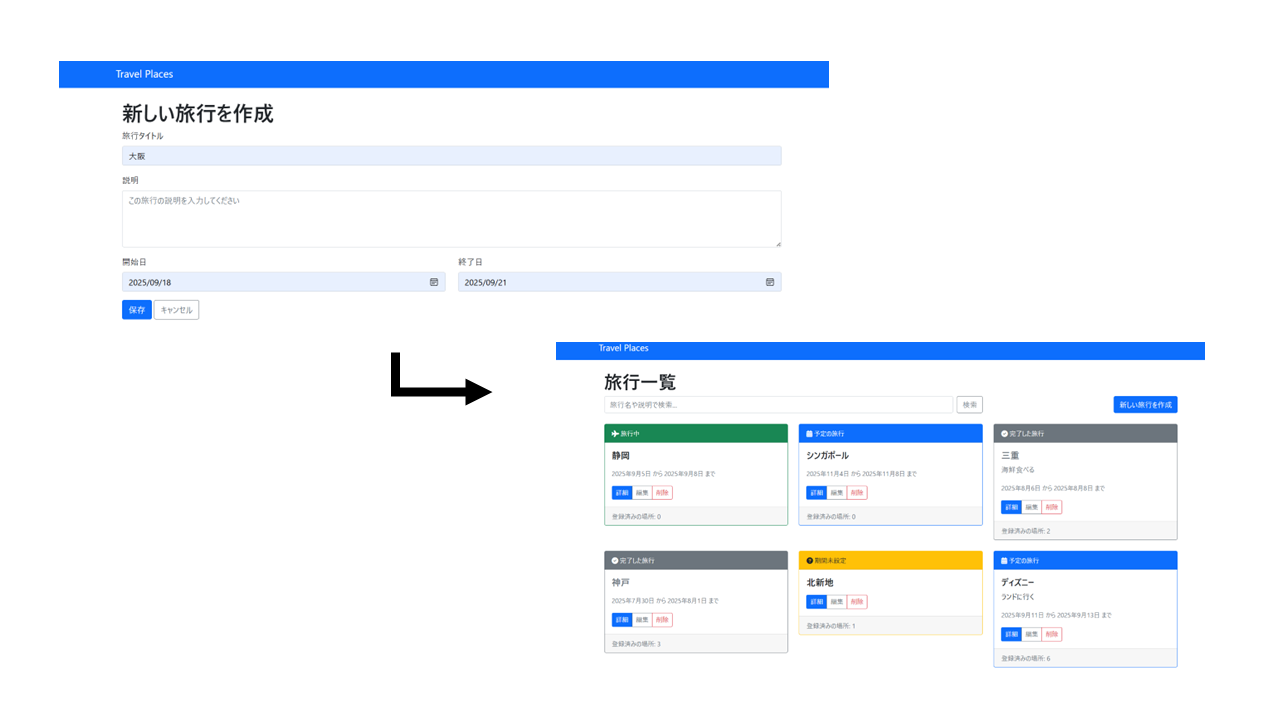
\includegraphics[width=10cm]{./figs/trip1.png}
\caption{\label{fig:orge3687c8}旅行日付に基づく時系列判定と色分けによる視覚的管理を行ったときの画面.}
\end{figure}


\section{今後の課題}
\label{sec:org4842f37}
今回は,旅行日数に応じた日程項目の自動生成,旅行日程に基づく色分け表示,キーワード検索機能を開発した.
今後は,更なるユーザビリティの向上のため,旅行準備の漏れを防ぐための持ち物チェックリスト機能や,日程に応じて柔軟に観光訪問順を変更できる入れ替え機能の開発を予定している.
これにより,旅行計画の精度向上を図る.


\small\setlength\baselineskip{10pt}
\begin{thebibliography}{9}

\bibitem{旅しお} 旅しお,\url{https://tabisio.com/},(2025/09/05 accessed).
\bibitem{Django}Djangoドキュメント,\url{https://docs.djangoproject.com/ja/5.1/topics/},(2025/09/05 accessed).
\bibitem{Django}Djangoの概要 ,\url{https://docs.djangoproject.com/ja/5.1/intro/overview/},(2025/09/05 accessed).
\end{thebibliography}
\end{document}
